\section{Question 1}
\subsection{1.1 Getting started}
\small
\begin{itshape}
Asynchronous updating of the nodes ensures that the dynamics of the Hopfield model with symmetric weights $w_{ij} = w_{ji}$ always converge to a fixed point. An energy function in this case is given by:
\begin{equation}
H(t)=-\sum_{i=1}^n \sum_{j=1}^n \omega_{ij} S_i(t) S_j(t)
\label{eq: energy function}
\end{equation}
Implement the Hopfield network as described above. Shortly comment on your implementation. The overlap of the network in state $S(t)$ with a given pattern $\psiμ$ is defined by $\frac{1}{N}\sum_{i=1}^N \psi_i^{mu} 	S_i(t)$. Set N = 200, P = 5, c = 0.2. For the first two unit time steps of the retrieval of one pattern, plot the changing values of the energy function and the overlap of the network with the pattern as the state of each node is sequentially updated.
\end{itshape}

\begin{wrapfigure}{r}{0.5\textwidth}
  \vspace{-20pt}
  \begin{center}
    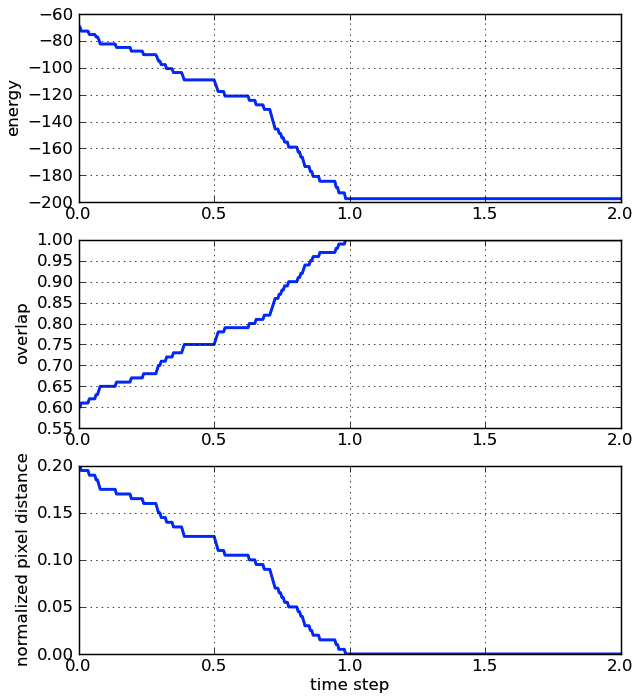
\includegraphics[width=0.48\textwidth]{img/plots/energy_overlap-1336935800.png}
  \end{center}
  \vspace{-20pt}
  \caption{Exercise 1	}
  \label{fig: Question 1.1}
  \vspace{-10pt}
\end{wrapfigure}
\paragraph*{}

\normalsize
The Hopfield Network was implemented and its source code can be found in the appendix. In order to execute it, one should first execute \texttt{h=HopfieldNetwork()} in order to initialize the class. Then one can execute the class using \texttt{h.run()}. The options of the \texttt{run} function are \texttt{N} (number of pixels), \texttt{P} (number of patterns), \texttt{ratio} (fraction of 1 in patterns), \texttt{mu} (pattern chosen for retrieval), \texttt{flip$\_$ratio} (fraction of pixels that are to be changed when creating the retrieval pattern), \texttt{pcut} (), \texttt{bPlot} (whether a plot should be created) and \texttt{bDebug} (whether debugging tools should be turned on).
By default the functio is set to \texttt{run(self, N=200, P=5, ratio=0.5, mu=0, flip$\_$ratio=0.2, pcut=0, bPlot=True, bDebug=False)}.
At first, the script only ran very slowly, this is because we did not have a lot of experience with python and thus used to for loops to do matrix multiplications. After implementing the \texttt{numpy.dot} function, the script ran incredibly much faster. 

\subsection{1.2 Normalized Pixel Distance}
\small
\begin{itshape}
Using the overlap defined in 1.1, derive an expression for the percentage of pixels in the network state $S$ which differ from the pattern $\psi^\mu$. This is the (normalized) pixel distance.
\end{itshape}

\paragraph*{}
\normalsize
Since the overlap gives the fraction of pixels which are identical between the network in state $S(t)$ and the pattern $\psi^\mu$, and the normalized pixel distance must be normalized to the domain $[0,1]$, it must be given by:

\begin{equation}
d=\frac{1- \frac{1}{N} \sum_{i=1}^N \xi_i^{mu} S_i(t)}{2}
\end{equation}

The normalized pixel distance was plotted together with the energy and the overlap in figure \ref{fig: Question 1.1}.

\subsection{1.3 Pattern retrieval}
\small
\begin{itshape}
We define the retrieval error of a pattern $\xi^\mu$ in a Hopfield network as the normalized pixel distance of the network state $S$ to the pattern $\xi^\mu$ after convergence, when retrieving the pattern $\xi^\mu$ as described above.

Set N = 200 and c = 0.1. Plot the mean retrieval error of a randomly chosen pattern averaged over different network realizations as a function of the dictionary size P. Average over enough network realizations to give a smooth curve and give error bars for the estimation of the mean (you can assume the variation to be normally distributed). From your data points and the chosen confidence interval, roughly estimate a maximal P at which patterns can be retrieved from the network with a mean retrieval error of less than 2$\%$?
\end{itshape}

\begin{wrapfigure}{r}{0.5\textwidth}
  \vspace{-20pt}
  \begin{center}
    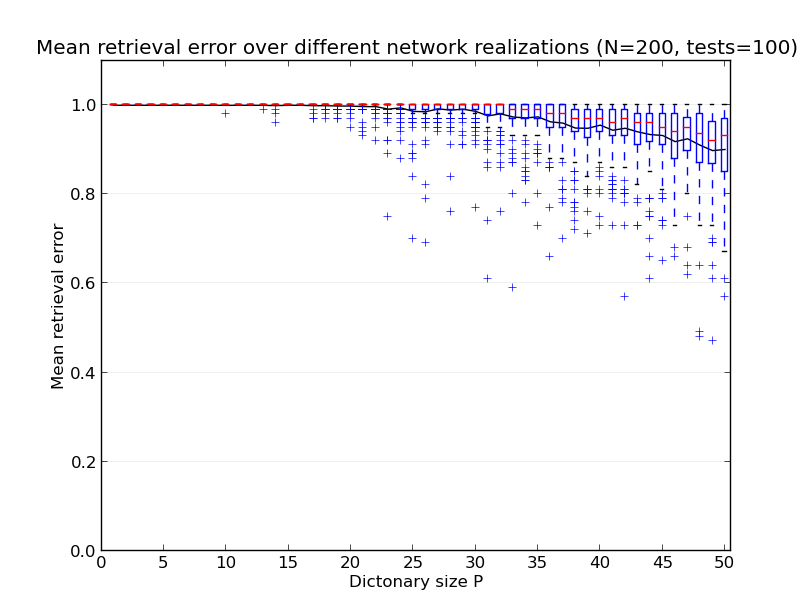
\includegraphics[width=0.6\textwidth]{img/plots/error-avg-100.png}
  \end{center}
  \vspace{-20pt}
  \caption{Exercise 1.3: Mean retrieval error averaged over 100 different network realizations.}
  \label{fig: Question 1.3}
  \vspace{-10pt}
\end{wrapfigure}
\paragraph*{}
Figure \ref{fig: Question 1.3} shows a plot of the mean retrieval error with respect to the dictionary size P. As one can see, the error remains very close to 0 for a dictionary size lower than 20. After that the error starts increasing. We have included a horizontal line at y = 0.02 indicating the 2$\%$ error. From that line, one would roughly estimate that the maximal P at which patterns can be retrieved is P=35. 

\section{Question 2}
\small
\begin{itshape}
We now define the capacity of a Hopfield network of size N as the number of patterns $P_{N,max}$ that
can be stored, such that the mean retrieval error averaged over all stored patterns (one retrieval
attempt each) is at most 2$\%$. This yields the maximal load $\alpha_{N,max} = \frac{P_{N,max} }{N}$.
Set c=0.1. Calculate $\alpha_{N,max}$ for at least 10 network realizations and state the mean together with confidence intervals. Do this for N = 100, 250 and one other larger network size. Shortly interpret the resulting values and compare with results from literature.
\end{itshape}

\begin{table}[H]
\centering
\begin{tabular}{|l|l|l|l|l|l|l|}
\hline
N & tests & C-level & maximal load & lower bound & upper bound & $P_{N,max}$\\ 
\hline
\hline
100 & 10 & 95$\%$ & 0.11600 & 0.11386 & 0.11815 & 11.6 \\
250 & 10 & 95$\%$ & - & - & - & - \\
500 & 10 & 95$\%$ & - & - & -  & -\\
\hline
\end{tabular}
\end{table}

